\section{Anwendung der Differential- und Integralrechnung}

\subsection{Beschreibungungsvarianten}
	\begin{minipage}[t]{3.5cm}
		Funktion (explizit) \\
		$ y = f(x)$ \\
        \tiny{(Bronstein S.49, 147)}
	\end{minipage}
	\begin{minipage}[t]{6cm} 		
		Koordinatengleichung (implizit) \\
		$ F(x,y) = 0 $ \\
        \tiny{(Bronstein S.49)}
	\end{minipage}
	\begin{minipage}[t]{5.5cm} 		
		Parameterform(Cartesisch) \\
		$ \left( \begin{array} {l} x(t) \\ y(t) \end{array} \right) =
          \left( \begin{array} {l} \Psi(t) \\ \varphi(t) \end{array} \right)$\\
        \tiny{(Bronstein S.49)}
	\end{minipage} 
	\begin{minipage}[t]{3cm}
    	Polarform x\\
    	$ r=f(\varphi) $ \\
    \end{minipage}\\

	$\rightarrow$ Ordnung immer ohne $\sqrt{\text{ }}$ \\

\subsection{Umrechnen diverser Systeme \formelbuch{49}}
\begin{tabular}{| l l | l|}
\hline Parameter 
	& $\Rightarrow$ explizit
	%& $x = f(t) \; \; y = g(t)$
	& $ t = f(x);\; y = g(f(x))$\\
\hline Explizit
	& $\Rightarrow$ Parameter
	%& $y = f(x)$
	& $ \left( \begin{array} {l} x(t) \\ y(t) \end{array} \right) =
          \left( \begin{array} {l} t \\ g(t) \end{array}
          \right)$ \\
\hline Ex- bzw. implizit 
	& $\Rightarrow$ Polar
	%& $y = f_1(x)$ bzw. $f_2(x,y) = C$
	&  Ersetze $x = r \cos(\varphi)$ ; $y = r \sin(\varphi)$ ; $x^2+y^2 = r^2$\\ 
\hline Polar 
	& $\Rightarrow$ implizit
	%& $r = f(\varphi)$
	& Ersetze $r \sin(\varphi) = y$; $r \cos(\varphi)=x$; $r=\sqrt{x^2 + y^2}$\\ 
\hline Polar
	& $\Rightarrow$ Parameterform
	%& $r = f(\varphi)$
	& $\left( \begin{array} {l} x(\varphi) \\ y(\varphi) \end{array} \right) =
          \left( \begin{array} {l} r(\varphi) \cos(\varphi) \\ r(\varphi) \sin(\varphi) \end{array}
          \right)$ \\
\hline Einzelner Punkt  
	& $\Rightarrow$ Polar
	%& $(x,\; y)$
	& $r = \sqrt{x^2 + y^2};\;
	\varphi = \begin{cases}\arctan(\frac{y}{x}) + \pi 	&x < 0\\
             \arctan(\frac{y}{x}) 	& x > 0\\
             \frac{\pi}{2}			& x = 0;\; y > 0\\
             -\frac{\pi}{2}			& x = 0;\; y < 0\\
             \text{unbestimmt}		& x = y = 0\end{cases}$\\
\hline
\end{tabular}

\subsection{Kurvenarten\formelbuch{203ff}}
$ \left.\begin{matrix}
	\text{bei `+`, Kurve auf linke Seite geöffnet}\\ 
	\text{bei `-`, Kurve auf rechte Seite geöffnet}
\end{matrix}\right\rbrace $ 
bei Polarform

\begin{tabular}{llll}
\parbox{2.7cm}{
\textbf{ } \\
Implizit:\\
Bemerkung:\\
Polarform:\\
Parameterform:\\
$p, \epsilon$:
}

\parbox{6cm}{
\textbf{Kreis\formelbuch{203}}\\
$(x-x_0)^2 + (y - y_0)^2 = r^2$\\
Mittelpunkt $(x_0, y_0)$; Radius $r$\\
$r = \frac{p}{1 + \epsilon \cos(\varphi)}; \epsilon = 0$\\
$x=x_0 + R\cos(t), y=y_0 + R\sin(t) $ \\
$ p = \frac{b^2}{a}$
} 

\parbox{8cm}{
\textbf{Ellipse\formelbuch{204}}\\
$(\frac{x-x_0}{a})^2 + (\frac{y-y_0}{b})^2 = 1$\\
Mittelpunkt $(x_0, y_0)$; Halbachsen $a$, $b$\\
$r = \frac{p}{1 + \epsilon \cos(\varphi)}; 0 < \epsilon < 1 \qquad$ (rechter Brennpunkt)\\
$x = a\cos(t), y = b\sin(t) \qquad$ um $P(0,0)$ \\
$\epsilon = \frac{c}{a}$
}\\ \\


\parbox{2.7cm}{
\textbf {}\\
Implizit:\\
Bemerkung:\\
Polarform:\\
Parameterform:
}

\parbox{6cm}{
\textbf{Hyperbel\formelbuch{206}}\\ 
$(\frac{x}{a})^2 - (\frac{y}{b})^2 = 1; -(\frac{x}{a})^2 + (\frac{y}{b})^2 =1$\\ 
Achsenkreuz in $P(0,0)$\\
$r = \frac{p}{1 - \epsilon \cos(\varphi)}; \epsilon > 1_{(rechter Hyperbelast)}$\\
$r = \frac{p}{1 + \epsilon \cos(\varphi)}_{(linker Hyperbelast)}$ \\
$x= a \cosh(t), y = b \sinh(t) $ 

}

\parbox{8cm}{
\textbf{Parabel\formelbuch{209}}\\
$y^2 = 2p(x-x_0)$\\
Parabeln mit Scheitelpunkt auf der vertikaler Achse\\
$r = \frac{p}{1 - \epsilon \cos(\varphi)}; \epsilon = 1$\\
$x= \frac{t^2}{2p}, y = t$\\
$p=$Halbparameter (2$\cdot$Abstand Scheitel-Brennpunkt)
}\\ \\

\parbox{2.7cm}{
\textbf{} \\
Polarform:
}

\parbox{5cm}{
\textbf{Kardioide/Herzk. \formelbuch{99}} \\
$r = a(1+\cos(\varphi))$
}

\parbox{5cm}{
\textbf{Lemniskate ``$\infty$'' \formelbuch{101}} \\
$r = a\sqrt{2\cos(2\varphi)}$ 
}

\parbox{5cm}{
\textbf{Strophoide/harm. K. \formelbuch{96}} \\
$ r = -a \frac{\cos(2\varphi)}{\cos(\varphi)},(a>0) $ 
}

\end{tabular}

\subsection{Gleichungen, Mittelwerte\formelbuch{19ff, 509}}
\begin{tabular}{llll}
	\textbf{Tangentengleichung} &
	\textbf{Normalengleichung} &
	\textbf{Linearer Mittelwert} &
	\textbf{Quadratischer Mittelwert}\\
	$y-y_0=f'(x_0)(x-x_0)$ &
	$y-y_0=-\frac{1}{f'(x_0)}(x-x_0)$ &
	$\bar{f} = \frac{1}{b-a} \int\limits_{a}^{b} f(x)dx$ &
	$\bar{f} = \sqrt{\frac{1}{b-a} \int\limits_{a}^{b} f(x)^2dx}$ \\
	$\dot{x_0}(y-y_0) = \dot{y_0}(x-x_0)$ \\
\end{tabular}
	
\subsection{Tangenten- \& Normalenabschnitt, Subtangente \& Subnormale\formelbuch{251ff}}

\subsection{Abstandsformeln}
\begin{tabular}{p{7cm}p{5cm}p{6cm}l}
	\textbf{Hessesche Normalform\formelbuch{200f, 224}} &
	\textbf{Geradengleichung} &
	\textbf{Abstand zum Ursprung} \\
	$x\cdot \cos\varphi_0 +y\cdot \sin\varphi_0=r_0$ &
	$y - y_0 = m (x - x_0)$ &
	$\frac{|y_0 - m \cdot x_0|}{\sqrt{m^2 + 1}}$ \\
	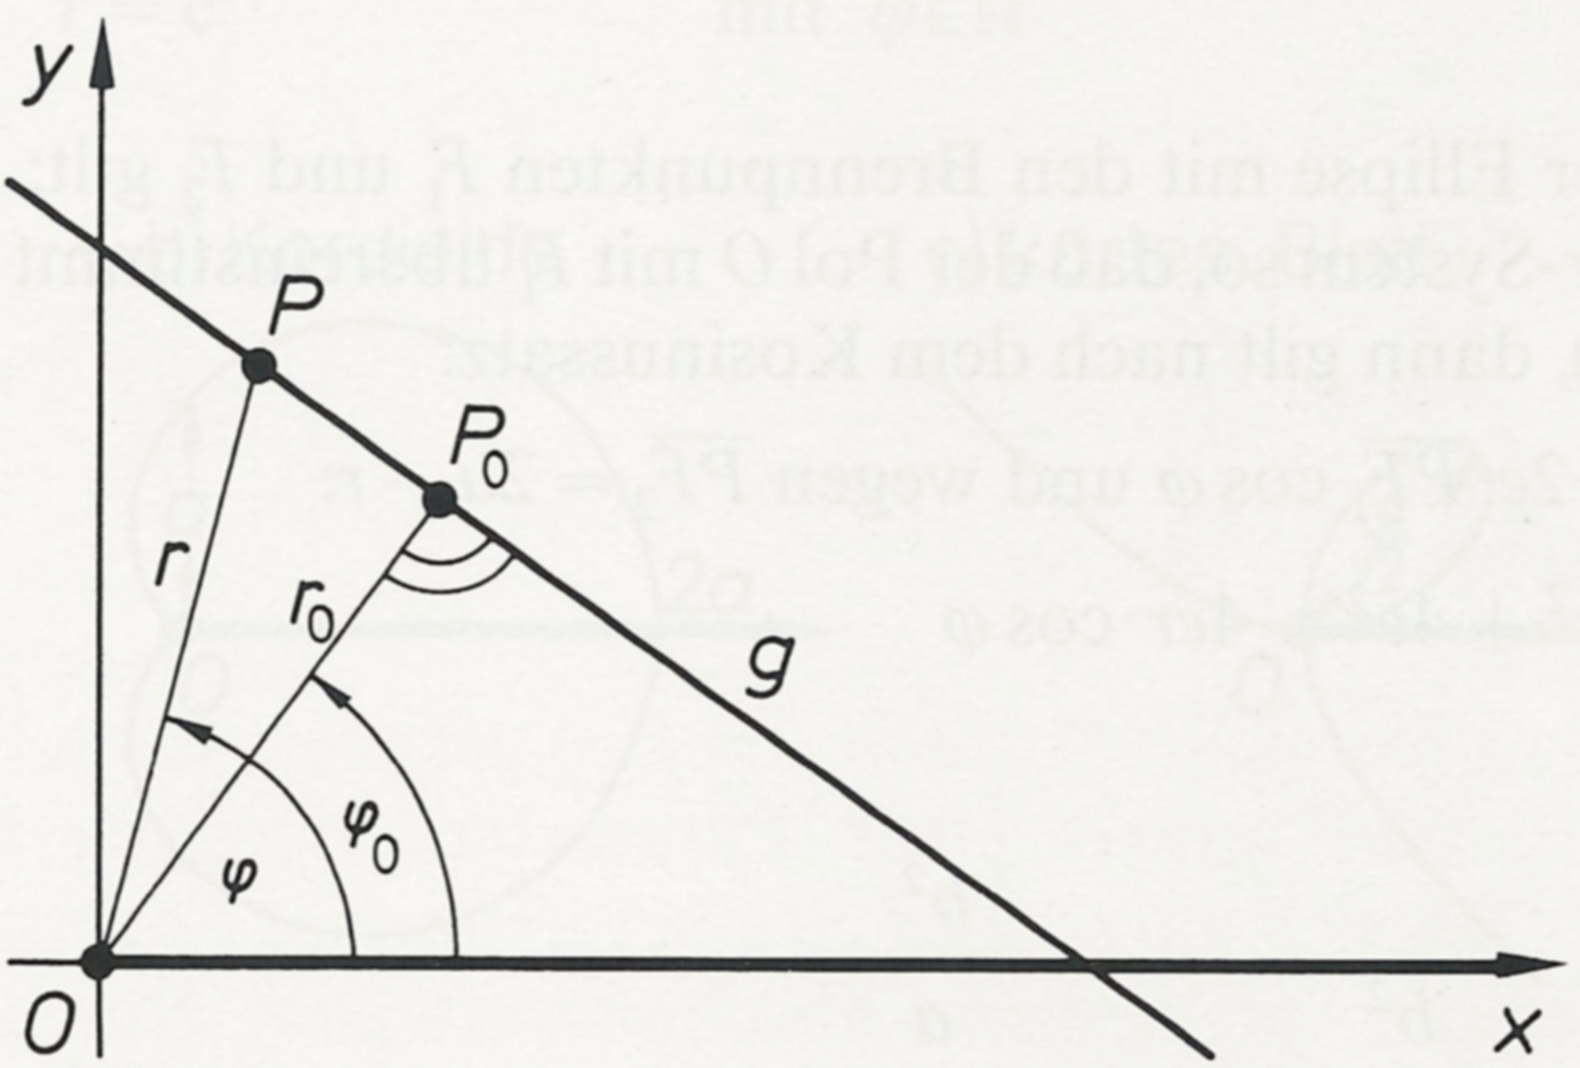
\includegraphics[width=6cm]{./bilder/hessenorm.png} \\
\end{tabular}


\subsection{Berührung in n-ter Ordnung}
Zwei explizit gegebene Kurven $y = f(x)$ und $y = g(x)$ berühren einander im
Punkt P $x_0, y_0$ von der Ordnung $n$, wenn die Funktionswerte und die ersten
$n$ Ableitungen existieren und übereinstimmen.\\
$f(x_0) = g(x_0);\; f'(x_0) = g'(x_0);\; f''(x_0) = g''(x_0);\;\ldots ;
\;f^{(n)}(x_0) = g^{(n)}(x_0)\; \qquad f^{(n+1)}(x_0) \neq g^{(n+1)}(x_0)$

\subsection{Scheitel \formelbuch{256}}
Scheitelpunte sind Extremalwerte der Krümmungs- bzw. Krümmungsradiusfunktion.
Falls bei $\kappa'(x)$ an der Stelle $x_0$ ein Vorzeichenwechsel besteht, existiert dort
eine Extremalstelle. 
$\qquad \kappa'(x) = 0; \kappa''(x) \neq 0$

\subsection{Wichtige Formeln\formelbuch{249ff}}
	\renewcommand{\arraystretch}{2}
	\begin{tabular}[c]{ | p{5.1cm} | p{5.4cm} | l | }
		\hline
		\textbf{Cartesisch} & \textbf{Parameter} & \textbf{Polar} \\
		\hline
		\multicolumn{3}{| l |}{\textbf{Anstieg einer Kurve, Ableitung, 2. Ableitung}} \\
    	\hline   
    	$y'=f'(x_o) \quad y'' = f''(x_0)$ & 
    	$y'=\frac{\dot{y}}{\dot{x}} \quad 
    	y'' = \frac{\dot{x} \ddot{y} - \dot{y}\ddot{x}}{\dot{x}^3}$ &
    	$y'=\frac{r'(\varphi) \sin(\varphi) + r(\varphi) \cdot
    	\cos(\varphi)}{r'(\varphi) \cos(\varphi)-r(\varphi) \cdot \sin(\varphi)}$
    	\\
		
		\hline
		\multicolumn{3}{| l |}{\textbf{Bogenlänge \formelbuch{514}}} \\
    	\hline
    	$s=\int\limits_a^b{\sqrt{1+(f'(x))^2}dx}$ & 
    	$|s|=\int\limits_{t_1}^{t_2}{\sqrt{\dot{x}^2(t)+\dot{y}^2(t)}dt}$ &
		$|s|=\int\limits_{\varphi_1}^{\varphi_2}{\sqrt{(r'(\varphi))^2+(r(\varphi))^2}d\varphi}$\\
		
		\hline		
		\multicolumn{3}{| l |}{\textbf{Krümmung ebener Kurven \formelbuch{253}}}\\
    	\hline
    	$\kappa=\frac{f''(x)}{(\sqrt{1+(f'(x))^2})^3}$ &
    	$\kappa=\frac{\dot{x}(t)\ddot{y}(t)-\dot{y}(t)\ddot{x}(t)}{(\sqrt{(\dot{x}(t))^2+(\dot{y}(t))^2})^3}$ &
		$\kappa=\frac{2(r'(\varphi))^2-r(\varphi)r''(\varphi)+(r(\varphi))^2}{(\sqrt{(r'(\varphi))^2+(r(\varphi))^2})^3}$\\   	
		
		\hline
		\multicolumn{3}{| l |}{Konvex (Linkskurve): $\kappa \geq 0 \qquad$ Streng
		konvex: $\kappa > 0 \qquad$ Wendepunkt: $\kappa = 0 \qquad$ Analog für konkav}\\
		
		\hline
		\multicolumn{3}{| l |}{\textbf{Krümmungskreisradius \formelbuch{253}} $\qquad r = |\frac{1}{\kappa}|$} \\
		\hline
		$r = \left|\frac{(\sqrt{1+(f'(x))^2})^3}{f''(x)} \right|$ &
		$r = \left|\frac{(\sqrt{(\dot{x}(t))^2+(\dot{y}(t))^2})^3}
		{\dot{x}(t)\ddot{y}(t)-\dot{y}(t)\ddot{x}(t)} \right|$ & 
		$r = \left|\frac{(\sqrt{(r'(\varphi))^2+(r(\varphi))^2})^3}
		{2(r'(\varphi))^2-r(\varphi)r''(\varphi)+(r(\varphi))^2} \right|$ \\
		
		\hline		
		\multicolumn{3}{| l |}{\textbf{Flächeninhalt \formelbuch{513}} um x-Achse /  für y-Achse: $f(y)$ von $y_0$ bis $y_1$ integrieren} \\
    	\hline
    	$A=\int\limits_a^b{f(x)}dx$  & 
    	$A=\frac{1}{2}\int\limits_{t_1}^{t_2}{[x(t)\dot{y}(t)-\dot{x}(t)y(t)]dt}$ &
		$A=\frac{1}{2}\int\limits_{\varphi_1}^{\varphi_2}{(r(\varphi))^2d\varphi}$\\  
    	
		\hline		
		\multicolumn{3}{| l |}{\textbf{Volumen \formelbuch{514}} um x-Achse 
		 / für y-Achse: $f(y)$ von $y_0$ bis $y_1$ integrieren
		 / Nur 1.Hälfte der Kurve integrieren!} \\
    	\hline
		$V=\pi\int\limits_a^b(f(x))^2dx$ & 
    	$V=\pi\left|\int\limits_{t_1}^{t_2}{(y(t))^2\dot{x}(t)dt}\right|$ &
		$V=\pi\left|\int\limits_{\varphi_1}^{\varphi_2}{r^2(\varphi)\sin^2\varphi[r'(\varphi)\cos(\varphi)-r(\varphi)\sin(\varphi)]d\varphi}\right|$\\  
    	
		\hline		
		\multicolumn{3}{| l |}{\textbf{Oberflächeninhalt \formelbuch{514}} um x-Achse 
		 / für y-Achse: $f(y)$ von $y_0$ bis $y_1$ integrieren
		 / Nur 1.Hälfte der Kurve integrieren!} \\
    	\hline
   		$O=2\pi\int\limits_a^b{|f(x)|\sqrt{1+(f'(x))^2}dx}$ & 
    	$O=2\pi\int\limits_{t_1}^{t_2}{|y(t)|\sqrt{\dot{x}^2(t)+(\dot{y}^2(t))}dt}$ &
		$O=2\pi\int\limits_{\varphi_1}^{\varphi_2}{|r(\varphi)\sin\varphi|\sqrt{(r'(\varphi))^2+(r(\varphi))^2}d\varphi}$\\  
    	\hline
		\multicolumn{3}{| l |}{Polar: \qquad $\sin \varphi =$ Drehung um Polgerade \qquad $\cos y =$ Drehung um y-Achse $(f = \frac{\pi}{2}) \qquad \rightarrow$ siehe Fläche} \\
	\hline
		\multicolumn{3}{| l |}{\textbf{Krümmungskreismittelpunkt}} \\
	\hline
		$x_c = x - \frac{\frac{dy}{dx}[1 + (\frac{dy}{dx})^2]}{\frac{d^2y}{dx^2}}$&
		$ x_c = x - \frac{\dot{y}(\dot{x}^2 + \dot{y}^2)}{\dot{x}\ddot{y} - \ddot{x}\dot{y}} $ &
		$x_c = r\cdot \cos\varphi - \frac{(r^2 + r'^2)(r\cdot \cos\varphi + r' \cdot \sin\varphi)}{r^2 + 2r'^2 - r\cdot r''}$\\

		$y_c = y + \frac{1+ (\frac{dy}{dx})^2}{\frac{d^2y}{dx^2}}$&
		$y_c = y + \frac{\dot{x}(\dot{x}^2 + \dot{y}^2)}{\dot{x}\ddot{y} - \ddot{x}\dot{y}} $ &
		$y_c = r\cdot \sin\varphi - \frac{(r^2 + r'^2)(r\cdot \sin\varphi - r' \cdot \cos\varphi)}{r^2 + 2r'^2 - r\cdot r''}$\\
	\hline
	\end{tabular}
	\renewcommand{\arraystretch}{1}
	
\subsection{Evolute}
Evolute = $\Sigma$ Krümmungskreiszentren\\
$\left(\begin{matrix} x_c \\ y_c \end{matrix}\right) = \left(\begin{matrix} x \\  y \end{matrix}\right) + \frac{1}{\kappa}\overrightarrow{n}$

\subsection{Orthogonaltrajektorien}
\begin{tabular}{ll}
\parbox{2.5cm}{
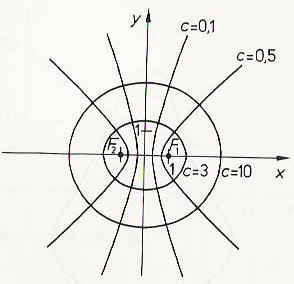
\includegraphics[height=2.5cm]{./bilder/orthoTrajekt.png}
}
& \parbox{16.5cm}{
Die orthogonalen Trajektorien schneiden alle Kurven der gegebenen Kurvenschar
$y=f(x,c)$ (c bestimmen) im rechten Winkel.
Die DGL $F(x,y,y')$ der Kurve bestimmen($y'$ ableiten, c einsetzen, wenn möglich für $f(x,c) = y$), anschliessend $y'$ durch
$-\frac{1}{y'}$ ersetzen.
$\Rightarrow$ ergibt die DGL der orthogonalen Trajektorien.\\
Die Kreise sind Orthogonaltrajektorien der Hyperbeln und umgekehrt.\\
$\frac{r'}{r} = f(\varphi , r) \qquad \underrightarrow{orthogonal}  \qquad \frac{r'}{r} = - \frac{1}{f(\varphi , r)}$
}
\end{tabular}

%%%%%%%%%%%%%%%%%%%%%%%%%%%%%%%%%%%%%%%%%%%%%%%%%%%%%%%%%%%%%%%%%%%%%%%%%%%%%%%%%%%%%%%%%%%%%%%%
%%%%%%%%%%%%%%%%%%%%%%%%%%%%%%%%%%%%%%%%%%%%%%%%%%%%%%%%%%%%%%%%%%%%%%%%%%%%%%%%%%%%%%%%%%%%%%%%
